\section{Descripción}


%%%%%%------Tableros-----%%%%%%
\subsection{Tableros}

\begin{frame}
    \frametitle{\insertsection}
    \framesubtitle{\hskip30pt \insertsubsection}

    \begin{block}{Tableros}
        \begin{itemize}
            \item\uncover<1->{Tamaño 10x10 casillas}
            \item\uncover<2->{Columnas identificadas con letras de la A - J}
            \item\uncover<3->{Filas numeradas del 1 al 10}
            \item\uncover<4->{Hay \textcolor{blue}{dos tableros:}}
                \begin{itemize}
                    \item\uncover<5->{\textbf{Tablero del jugador:} Donde el jugador coloca sus barcos y se registran
                    los disparos de la máquina.}
                    \item\uncover<6->{\textbf{Tablero del contrincante:} Donde la máquina coloca sus barcos y donde el jugador realiza sus disparos.}
                \end{itemize}
    \end{itemize}
    \end{block}
\end{frame}

\begin{frame}

    \begin{figure}
      \scalebox{0.34}{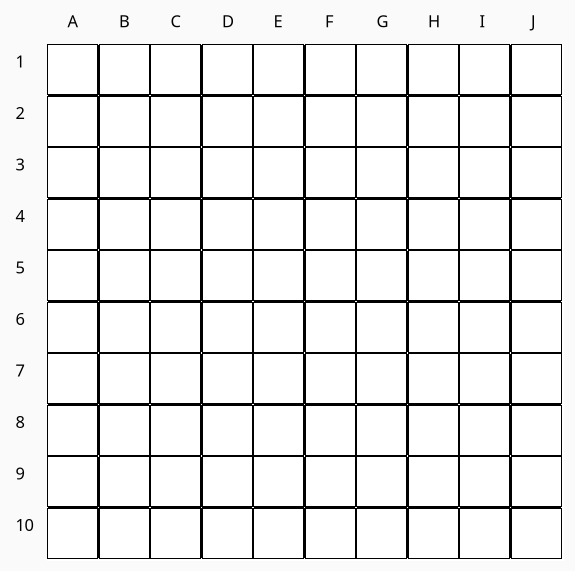
\includegraphics{imagenes/tablero.png}}
      \caption{Representación gráfica de un tablero}
    \end{figure}
\end{frame}


\subsection{Flota y restricciones en la colocación}

\begin{frame}
    \frametitle{\insertsection}
    \framesubtitle{\hskip30pt \insertsubsection}

    \begin{block}{Flota}
        \begin{itemize}
            \item\uncover<1->{1 x \textcolor{steelblue}{Portaaviones} de 5 casillas}
            \item\uncover<2->{1 x \textcolor{crimson}{Acorazado} de 4 casillas}
            \item\uncover<3->{ 2 x \textcolor{lightgreen}{Crucero} de 3 casillas}
            \item\uncover<4->{ 3 x \textcolor{darkkhaki}{Destructor} de 2 casillas}
            \item\uncover<5->{3 x \textcolor{navyblue}{Submarino} de 1 casilla}
        \end{itemize}
    \end{block}


\begin{figure}[h]
    \begin{columns}[c]
        
        \begin{column}{.2\textwidth}
            \centering
            \scalebox{0.4}{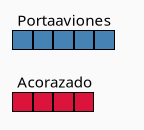
\includegraphics{imagenes/Barco1.png}}
        \end{column}

        \begin{column}{.2\textwidth}
            \centering
                \scalebox{0.34}{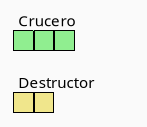
\includegraphics{imagenes/Barco2.png}}
        \end{column}

        \begin{column}{.2\textwidth}
            \centering
                \scalebox{0.34}{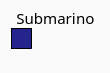
\includegraphics{imagenes/Barco3.png}}
        \end{column}
   
    \end{columns}
    \caption{Representación de la flota}
\end{figure}

\end{frame}


\begin{frame}
    \begin{block}{Restricciones en la colocación de los barcos}
        \begin{itemize}
            \item\uncover<1->{ Se pueden colocar vertical u horizontalmente.}
            \item\uncover<2->{\textcolor{red}{No} se permiten casillas con barco \textcolor{red}{contiguas} (ni diagonalmente).}
        \end{itemize}
    \end{block}


\begin{figure}
    \begin{columns}[c]
        
        \begin{column}{.3\textwidth}
            \centering
            \scalebox{0.28}{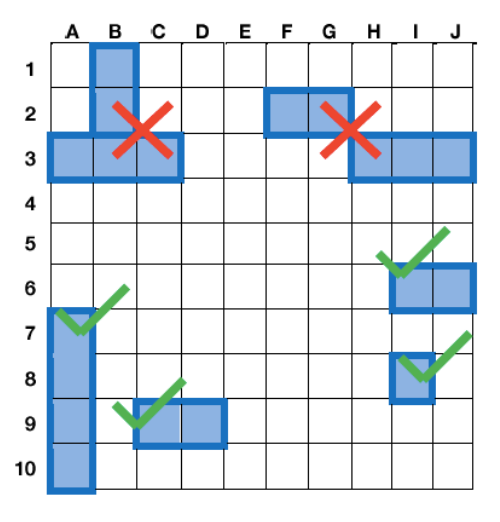
\includegraphics{imagenes/colocacionbarcos.png}}
        \end{column}
        \begin{column}{.3\textwidth}
            \centering
            \caption{Restricciones en la colocación}
        \end{column}
    \end{columns}
\end{figure}

\end{frame}


\subsection{Condición de victoria}

\begin{frame}
    \frametitle{\insertsection}
    \framesubtitle{\hskip30pt \insertsubsection}

    \begin{block}{Condición de victoria}
        Gana el primer jugador que \textcolor{blue}{hunda la flota} del contrincante.
    \end{block}
    
\end{frame}

\subsection{Contrincante}

\begin{frame}
    \frametitle{\insertsection}
    \framesubtitle{\hskip30pt \insertsubsection}

    \begin{block}{Contrincante}
        \begin{itemize}
            \item\uncover<1->{El único oponente será la \textcolor{blue}{CPU} (máquina).}
            \item\uncover<2->{Habrá tres tipos de algoritmos diferentes que podrá usar:}
            \begin{itemize}
                \item\uncover<3->{\textbf{Algoritmo aleatorio}}
                \item\uncover<4->{\textbf{Algoritmo Hunt/Target}}
                \item\uncover<5->{\textbf{Algoritmo Hunt/Target probabilístico}} 
            \end{itemize}
        \end{itemize}
    \end{block}
    
\end{frame}

\subsubsection{Algoritmo aleatorio}

\begin{frame}
    \frametitle{\insertsection}
    \framesubtitle{\hskip30pt \insertsubsection}

    \begin{block}{\textcolor{red}{Algoritmo aleatorio}}

        \begin{itemize}
            \item\uncover<1->{Realiza el disparo escogiendo una fila y una columna de forma aleatoria.}
            \item\uncover<2->{No escogerá casillas \textcolor{blue}{disparadas con anterioridad} o \textcolor{purple}{casillas contiguas} a barcos hundidos.}
        \end{itemize}
        
    \end{block}

    \begin{block}{Debilidades}
        \begin{itemize}
            \item\uncover<3->{Cuando un barco es alcanzado, el algoritmo no termina de hundirlo.}
            \item\uncover<4->{Recorre la mayoría de las casillas del tablero (muy ineficiente).}
        \end{itemize}
    \end{block}
\end{frame}

% \begin{frame}
%     \begin{figure}
%         \scalebox{0.34}{\includegraphics{imagenes/algoritmoAleatorio.gif}}
%         \caption{Representación gráfica de un tablero}
%       \end{figure}
% \end{frame}



\subsubsection{Algoritmo Hunt/Target}

\begin{frame}
    \frametitle{\insertsection}
    \framesubtitle{\hskip30pt \insertsubsection}

    \begin{block}{\textcolor{red}{Algoritmo Hunt/Target}}
        \begin{itemize}
            \item\uncover<1->{Usa \textcolor{red}{dos modos} (\textit{funciones}) alternos que usan una lista de objetivos conjuntamente para determinar la posición de un barco y hundirlo:}
            \begin{itemize}
                \item\uncover<2->{\textbf{Modo hunt} para buscar un objetivo}
                \item\uncover<3->{\textbf{Modo target} para hundir el barco}
            \end{itemize}
        \end{itemize}
    \end{block}
    
\end{frame}

\begin{frame}
    \frametitle{\insertsection}
    \framesubtitle{\hskip30pt \insertsubsection}

    \begin{block}{Modo Hunt}
        \begin{itemize}
            \item\uncover<1->{Dispara aleatoriamente una de las casillas del tablero que cumplan:}
            \begin{itemize}
                \item\uncover<2->{\textcolor{red}{no} disparadas con anterioridad ni contiguas a barcos hundidos.}
                \item\uncover<3->{\textcolor{blue}{pariedad par} y \textcolor{purple}{espacio} disponible para el barco de menor longitud sin hundir.}
            \end{itemize}
            \item\uncover<4->{Si el disparo es sobre un \textcolor{red}{barco}, se crea una \textcolor{darkcerulean}{lista con sus casillas vecinas} N - S - E - O}
        \end{itemize}
        
    \end{block}
\end{frame}

\begin{frame}
    \begin{block}{Pariedad par}
        Que casillas (mínimas) debe contener parte de un barco colocado de cualquier forma en el tablero.   
    \end{block}

    \begin{block}{Nota}
        Se aplica para el \textcolor{blue}{barco de menor longitud sin hundir} para garantizar tocar a todos los barcos en menos disparos.
    \end{block}
        
\end{frame}

\begin{frame}
    \begin{figure}
        \begin{columns}[c]
            
            \begin{column}{.5\textwidth}
                \centering
                \scalebox{0.30}{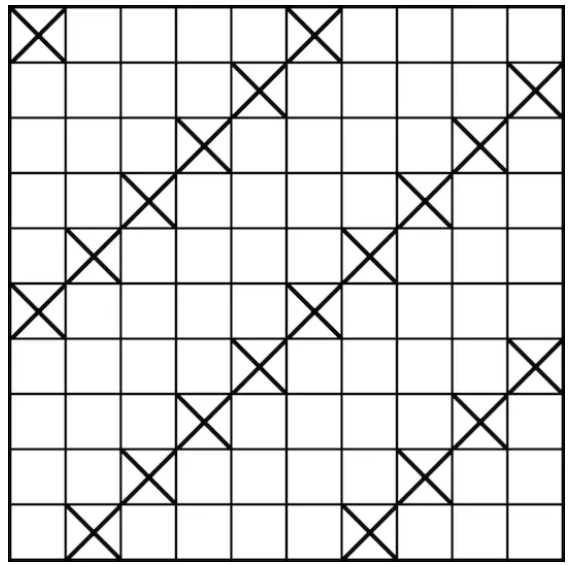
\includegraphics{imagenes/pariedad.png}}
            \end{column}
            \begin{column}{.3\textwidth}
                \centering
                \caption{Patrón de disparo para un barco de 5 casillas}
            \end{column}
        \end{columns}
    \end{figure}
\end{frame}

\begin{frame}
    \begin{block}{Espacio disponible}
        La casilla seleccionada debe contener al menos \textcolor{blue}{una dirección con suficientes casillas vacías} para albergar el barco
        de menor longitud sin hundir.
    \end{block}

\end{frame}

\begin{frame}
    \frametitle{\insertsection}
    \framesubtitle{\hskip30pt \insertsubsection}

    \begin{block}{Modo target}
        \begin{itemize}
            \item\uncover<1->{Dispara a las casillas de la \textcolor{blue}{lista objetivos} para precisar la \textcolor{red}{orientación} del barco:}
            \begin{itemize}
                \item\uncover<2->{Si el disparo es en la misma fila: \textcolor{purple}{horizontal}.}
                \item\uncover<3->{Si el disparo es en la misma columna: \textcolor{blue}{navyblue}.}
            \end{itemize}
            \item\uncover<4->{Una vez precisada la orientación, por cada acierto, se añade a la lista de objetivos la \textcolor{blue}{siguiente casilla} de la misma fila (horizontal) o de la misma columna (vertical).}
            \item\uncover<5->{Una vez que el barco es \textcolor{red}{hundido}, se vuelve al modo hunt para repetir el proceso.}
        \end{itemize}
    \end{block}

\end{frame}

\begin{frame}
    
    \begin{block}{Notas sobre la \textcolor{blue}{lista de objetivos}}
        \begin{itemize}
            \item\uncover<1->{Hay que \textit{barajarla} al principio para que los barcos verticales no tengan desventaja.}
            \item\uncover<2->{Es necesaria para \textcolor{green}{guardar los objetivos} después de un cambio de turno, o retroceder si el disparo no ha sido en los extremos}
            \item\uncover<3->{\textcolor{red}{Solo} contiene casillas no disparadas ni contiguas a barcos hundidos y dentro de los límites del tablero.}
        \end{itemize}
        
    \end{block}
\end{frame}

\begin{frame}
    \begin{block}{Fortalezas}
        \begin{itemize}
            \item\uncover<1->{Cuando un barco es alcanzado es hundido.}
            \item\uncover<2->{Se realizan menos disparos (es más eficiente).}
            \item\uncover<3->{Durante la evolución de la partida, el algoritmo es más rápido en hundir barcos.}
        \end{itemize}
    \end{block}
    \uncover<3->{\begin{block}{Debilidades}
        \begin{itemize}
            \item\uncover<3->{Todavía sigue usando aleatoriedad.}
            \item\uncover<4->{Necesita una lista de objetivos.}
            \item\uncover<5->{Al existir el barco de una casilla, en la mayoría de partidas el modo hunt no se beneficia de sus filtros.}
        \end{itemize}
    \end{block}}
\end{frame}

\subsubsection{Algoritmo Hunt/Target probabilístico}

\begin{frame}
    \frametitle{\insertsection}
    \framesubtitle{\hskip30pt \insertsubsection}

    \begin{block}{\textcolor{red}{Algoritmo Hunt/Target probabilístico}}
        \begin{itemize}
            \item\uncover<1->{Usa la \textcolor{blue}{misma idea} de los dos \textit{modos} que el algoritmo Hunt/Target normal.}
            \item\uncover<2->{\textcolor{red}{Mejora} el modo hunt y modo target para eliminar la \textit{aleatoriedad}.}
            \item\uncover<3->{Se mantiene el uso de la lista de objetivos}
            \item\uncover<4->{Se usan las \textit{\textbf{funciones de densidad de probabilidad}} para tomar las decisiones.}
        \end{itemize}
    \end{block}

    \uncover<5->{\begin{block}{Nota}
        Se puede usar una versión de este algoritmo sin lista de objetivos. Todas las decisiones serían
        tomadas con probabilidad.

    \end{block}}
    
\end{frame}

\begin{frame}
    \frametitle{\insertsection}
    \framesubtitle{\hskip30pt \insertsubsection}

    \begin{block}{Funciones de densidad de probabilidad} 
        \begin{itemize}
            \item\uncover<1->{Se considera que en el centro del tablero habrá más \textcolor{red}{densidad de barcos.}}
            \item\uncover<2->{Por cada casilla que haya un barco se asigna un \textbf{\textit{peso}.}}
            \item\uncover<3->{Se calculan todas las posibles posiciones en todas las casillas con todos los barcos \textcolor{purple}{(\textit{superposición})}}
            \item\uncover<4->{Al sumarse los pesos por cada posible variación en cada casilla, se obtiene una \textcolor{blue}{matriz de probabilidades.}}
        \end{itemize}    
    \end{block}


\end{frame}

\begin{frame}
    \begin{figure}
        \scalebox{0.4}{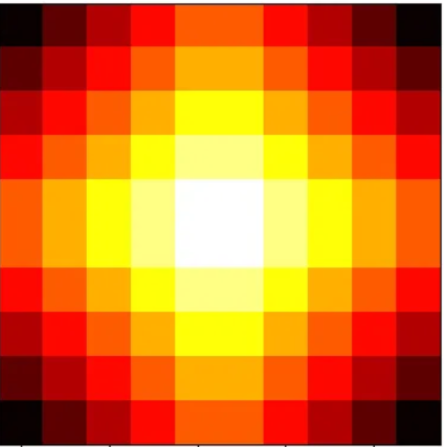
\includegraphics{imagenes/mapaCalorPortaaviones.png}}
        \caption{Ejemplo de representación de la matriz de probabilidad en un mapa de calor para un portaaviones}
      \end{figure}
\end{frame}

\begin{frame}
    \begin{figure}
        \scalebox{0.4}{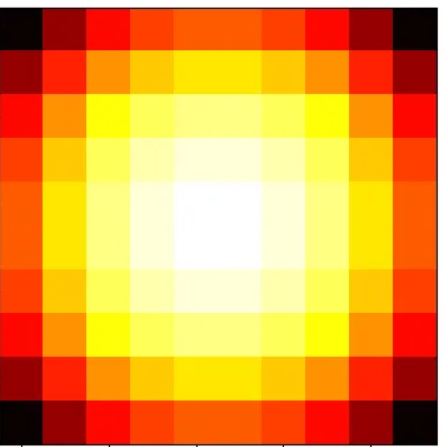
\includegraphics{imagenes/flotaMapa.png}}
        \caption{Ejemplo de representación de la matriz de probabilidad en un mapa de calor con todos los barcos}
      \end{figure}
\end{frame}

\begin{frame}
    \frametitle{\insertsection}
    \framesubtitle{\hskip30pt \insertsubsection}

    \begin{block}{Modo Hunt}
        \begin{itemize}
            \item\uncover<1->{Al principio, la \textcolor{blue}{matriz de probabilidades} es actualizada.}
            \begin{itemize}
                \item\uncover<2->{Las casillas disparadas o contiguas a barcos hundidos tendrán \textcolor{red}{probabilidad 0.}}
                \item\uncover<3->{Al calcular todas las posibles posiciones de los barcos, estos \textcolor{red}{no} pueden superponerse en casillas disparadas o contiguas a barcos hundidos.}
            \end{itemize}
            \item\uncover<4->{El objetivo será aquella casilla con \textcolor{blue}{mayor probabilidad.}}
            \begin{itemize}
                \item\uncover<5->{Si el disparo \textcolor{red}{falla}, se volverá a intentar con la siguiente mayor en el siguiente turno.}
                \item\uncover<6->{Si el disparo \textcolor{blue}{acierta}, se añaden las casillas vecinas a la lista de objetivos y se pasa el relevo al \textcolor{purple}{modo target.}}
            \end{itemize}
            
        \end{itemize}
    \end{block}
    
\end{frame}

\begin{frame}
    \frametitle{\insertsection}
    \framesubtitle{\hskip30pt \insertsubsection}

    \begin{block}{Modo Target}
        \begin{itemize}
            \item\uncover<1->{Usa la misma lógica que el modo target anterior.}
            \item\uncover<2->{La matriz de probabilidades es usada para decidir en que orden disparar sobre las casillas vecinas.}
            \item\uncover<3->{Si el disparo es sobre agua, se vuelven a calcular las probabilidades para elegir la casilla con mayor probabilidad.}
            \item\uncover<4->{Cuando la orientación es elegida, se actúa de la forma anterior (no se usa la matriz de probabilidades).}
        \end{itemize}
    \end{block}
    
\end{frame}

\begin{frame}
    \begin{block}{Fortalezas}
        \begin{itemize}
            \item\uncover<1->{Si la flota es colocada aleatoriamente (densidad alta en el centro), el \textcolor{red}{algoritmo es muy eficaz}}
            \item\uncover<2->{Permite ajustar la estrategia cambiando artificialmente los pesos según se desee}
            \item\uncover<3->{\textcolor{blue}{Fácilmente adaptable} para algoritmos más avanzados (Machine Learning)}
        \end{itemize}
    \end{block}
    \uncover<3->{\begin{block}{Debilidades}
        \begin{itemize}
            \item\uncover<4->{Usa una \textcolor{red}{estructura de datos auxiliar} extra (matriz de probabilidades).}
            \item\uncover<5->{Supone un gasto mayor en recursos en calcular cada vez la matriz de probabilidades.}
            \item\uncover<6->{Es \textcolor{red}{débil} si los barcos son colocados alejados del centro.}
        \end{itemize}
    \end{block}}
\end{frame}